
\subsection{Computational DAG}

A parallel program maybe be represented as a directed acyclic graph (DAG),
this graph has several properties, such as the span,
which can be used to evaluate the potential performance of an algorithm.

\begin{figure}[h]
    \centering
    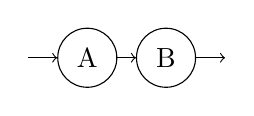
\begin{tikzpicture}
        \node[name=a, draw, circle, minimum size=0.75cm] at (0,0) {A};
        \node[name=b, draw, circle, minimum size=0.75cm] at (1,0) {B};
        \draw[->] (-.75, 0) -- (a);
        \draw[->] (a) -- (b);
        \draw[->] (b) -- (1.75,0);
    \end{tikzpicture}
    \caption{Serial Composition}
    \label{fig:dag:serial}
\end{figure}[h]


\begin{figure}[h]
    \centering
    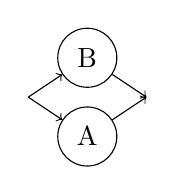
\begin{tikzpicture}
        \node[name=a, draw, circle, minimum size=0.75cm] at (0,0) {A};
        \node[name=b, draw, circle, minimum size=0.75cm] at (0,1) {B};
        \draw[->] (-.75, 0.5) -- (a);
        \draw[->] (-.75, 0.5) -- (b);
        \draw[->] (a) -- (.75, 0.5);
        \draw[->] (b) -- (.75, 0.5);
    \end{tikzpicture}
    \caption{Parallel Composition}
    \label{fig:dag:parallel}
\end{figure}[h]

\paragraph{Work}

The total number of tasks of the graph is called \textit{work},
this is equivalent to running the algorithm with a single processing unit ($T_1$).

\begin{equation}\label{eq:work_law}
    T_p \ge \frac{T_1}{P}
\end{equation}

The work is equal whether considering $T_1$ or $T_P$,
that is:

\begin{equation}
    T_1 (A \cup B) = T_1(A) + T_1(B)
\end{equation}

\paragraph{Span}

The span, or the critical-path length, is the minimum of sequential steps the algorithm must execute.

\begin{equation}\label{eq:span_law}
    T_p \ge T_{\infty}
\end{equation}

The span is different when comparing $T_1$ and $T_P$.

\begin{equation}
    \begin{split}
        T_{\infty} (A \cup B) & = T_{\infty}(A) + T_{\infty}(B)\\
        T_{\infty} (A \cup B) & = max\{T_{\infty}(A), T_{\infty}(B)\}\\
    \end{split}
\end{equation}

\subsubsection{Speedup}

The speedup on $P$ processors is given by:

\begin{equation}
    \frac{T_1}{T_P}
\end{equation}

If $\frac{T_1}{T_P} = P$ we have \textit{linear} speedup.
When $\frac{T_1}{T_P} \ge P$ we have \textit{superlinear} speedup,
this however is not possible due to the work law (\autoref{eq:work_law}).

\subsubsection{Parallelism}

Parallelism can be defined as the average amount of work per step along the span, that is:

\begin{equation}
    \frac{T_1}{T_\infty}
\end{equation}

\subsubsection{Work-Span Model}

Considers a greedy scheduler, that is,
no worker is idle while there are tasks to execute.

\begin{itemize}
    \item $T_P$ - running time with $P$ workers.
    \item $T_1$ - running time with 1 worker, serial execution.
    \item $T_\infty$ - the time taken along the critical path.
\end{itemize}

The critical path is the sequence of tasks that has the longest execution time.

\paragraph{Lower-Bound}
A lower-bound can be calculated with the following formula:

\begin{equation}
    \mathnormal{max}\left(\frac{T_1}{P}, T_\infty\right) \le T_P
\end{equation}

\paragraph{Upper-Bound}

\begin{equation}
    T_P \le \frac{T_1 - T_\infty}{P + T_\infty}
\end{equation}